\documentclass[12pt]{article}
%%% DOCUMENT FORMATTING %%%
\usepackage[margin=1in]{geometry}
\usepackage{enumitem}
\setlength{\parindent}{0pt}
\newcommand{\disp}{\displaystyle}

%%% HEADER %%%
\usepackage{fancyhdr}
\pagestyle{fancy}
\fancyhf{}
\lhead{MATH 1060}
\rhead{Vagnozzi}
\cfoot{\thepage}

%%% MATH NOTATION & SYMBOLS %%%
\usepackage{amssymb}
\usepackage{amsmath}
\newcommand{\R}{\mathbb{R}}
\newcommand{\N}{\mathbb{N}}
\newcommand{\Z}{\mathbb{Z}}
\newcommand{\lp}{\left(}
\newcommand{\rp}{\right)}
\newcommand{\ls}{\left[}
\newcommand{\rs}{\right]}
\newcommand{\lb}{\left\{}
\newcommand{\rb}{\right\}}
\newcommand{\arccot}{\text{arccot}}
\newcommand{\arccsc}{\text{arccsc}}
\newcommand{\arcsec}{\text{arcsec}} 

%%% TABLES %%%
\usepackage{colortbl}

%%% GRAPHS %%%
\usepackage{tikz}
\usepackage{pgfplots}
\pgfplotsset{compat=1.15}
\usepgfplotslibrary{fillbetween}
\usetikzlibrary{angles,quotes}

%%% ENVIRONMENTS %%%
\newcommand{\Example}{\paragraph{\Writinghand \hspace{0.1mm} Example.}}
\newcommand{\ExampleCont}{\paragraph{\Writinghand \hspace{0.1mm} Example (continued).}}
\newcommand{\boxenv}[2]{
	\fbox{
	\begin{minipage}{0.97\textwidth}
	\vspace{2mm}	
	\paragraph{#1} #2
	\vspace{2mm}
	\end{minipage}
	}}

%%% FUN THINGS %%%
\newcommand*\tc[1]{\tikz[baseline=(char.base)]{
            \node[shape=circle,draw,inner sep=2pt] (char) {#1};}}
\usepackage{marvosym}

%%% MISC %%%
\usepackage{hyperref}


\setcounter{page}{8}

\begin{document}
\section*{1.4: Trig and Inverse Trig Functions}

\boxenv{Learning Objectives.}{Upon successful completion of Section 1.4, you will be able to\dots
		
	\begin{itemize}[leftmargin=6mm]
		\item Answer conceptual questions involving trigonometric functions and their inverses.
		\item Evaluate trigonometric functions.
		\item Solve trigonometric equations.
		\item Evaluate inverse trigonometric functions.
		\item Graph trigonometric functions (i.e. a general sketch).
	\end{itemize}
	\vspace{-4mm}
}

\vspace{5mm}

\subsection*{Trigonometric Functions}
\paragraph{Right-Triangle Trigonometry.} Right triangles possess ratios that depend only on the central angle of the triangle, denoted here as $\theta$. 

\begin{center}
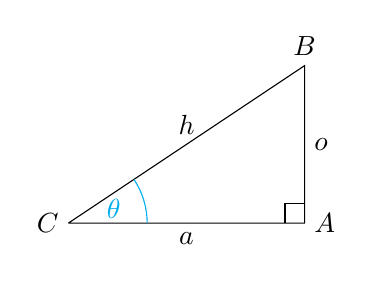
\begin{tikzpicture}[
  my angle/.style={
    every pic quotes/.append style={text=cyan},
    draw=cyan,
    angle radius=1cm,
  }]
  \coordinate [label=left:$C$] (C) at (-1.5,-1);
  \coordinate [label=right:$A$] (A) at (1.5,-1);
  \coordinate [label=above:$B$] (B) at (1.5,1);
  \draw (C) -- node[above] {$h$} (B) -- node[right] {$o$} (A) -- node[below] {$a$} (C);
  \draw (A) +(-.25,0) |- +(0,.25);
  \pic [my angle, "$\theta$"] {angle=A--C--B};
  %\pic [my angle, "$\beta$"] {angle=C--B--A};
\end{tikzpicture}
\end{center}

These ratios are \textbf{functions} of the central angle and have their own names: sine, cosine, tangent, cosecant, secant, and cotangent. Sine, cosine, and tangent are defined below.

\begin{center}
\begin{tabular}{|ccccccc|}
\hline
& & & & & & \\
& $\sin\theta=\disp\frac{o}{h}$ & & $\cos\theta=\disp\frac{a}{h}$ & & $\tan\theta=\disp\frac{o}{a}=\frac{\sin\theta}{\cos\theta}$ & \\
& & & & & & \\
\hline
\end{tabular}
\end{center}

Cosecant, secant, and cotangent are known as \textbf{reciprocal} trig functions. 

\begin{center}
\begin{tabular}{|ccccccc|}
\hline
& & & & & & \\
& $\csc\theta=\disp\frac{1}{\sin\theta}=\frac{h}{o}$ & & $\sec\theta=\disp\frac{1}{\cos\theta}=\frac{h}{a}$ & & $\cot\theta=\disp\frac{1}{\tan\theta}=\frac{a}{o}$ & \\
& & & & & & \\
\hline
\end{tabular}
\end{center}

Be careful not to confuse reciprocal trig functions with \textit{inverse} trig functions, defined later.

\vspace{3mm}

\boxenv{Remark.}{Note that, as with other functions, trigonometric functions must always have an argument (i.e.\ a function input). Writing ``$\sin$,'' ``$\cos$,'' or ``$\tan$'' with no argument does not convey any mathematical meaning.}

\newpage

\Example Write the six trig ratios for the following triangle.

\vspace{5mm}

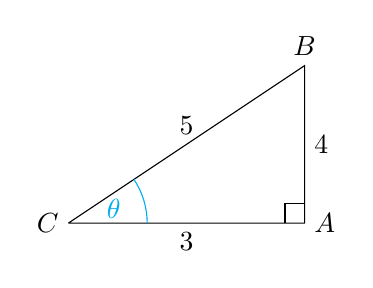
\begin{tikzpicture}[
  my angle/.style={
    every pic quotes/.append style={text=cyan},
    draw=cyan,
    angle radius=1cm,
  }]
  \coordinate [label=left:$C$] (C) at (-1.5,-1);
  \coordinate [label=right:$A$] (A) at (1.5,-1);
  \coordinate [label=above:$B$] (B) at (1.5,1);
  \draw (C) -- node[above] {$5$} (B) -- node[right] {$4$} (A) -- node[below] {$3$} (C);
  \draw (A) +(-.25,0) |- +(0,.25);
  \pic [my angle, "$\theta$"] {angle=A--C--B};
  %\pic [my angle, "$\beta$"] {angle=C--B--A};
\end{tikzpicture}

\vspace{5mm}

\textbf{The Unit Circle.} The \textbf{unit circle} is the circle with radius 1 that is centered at the origin. The coordinates of a unit circle are given by $\lp\cos(\theta),\sin(\theta)\rp$ for each $\theta$. %In other words, for each angle $\theta$, the $x$-coordinate represents the \textit{cosine} of that angle and the $y$-coordinate represents the \textit{sine} of the angle.

\begin{center}
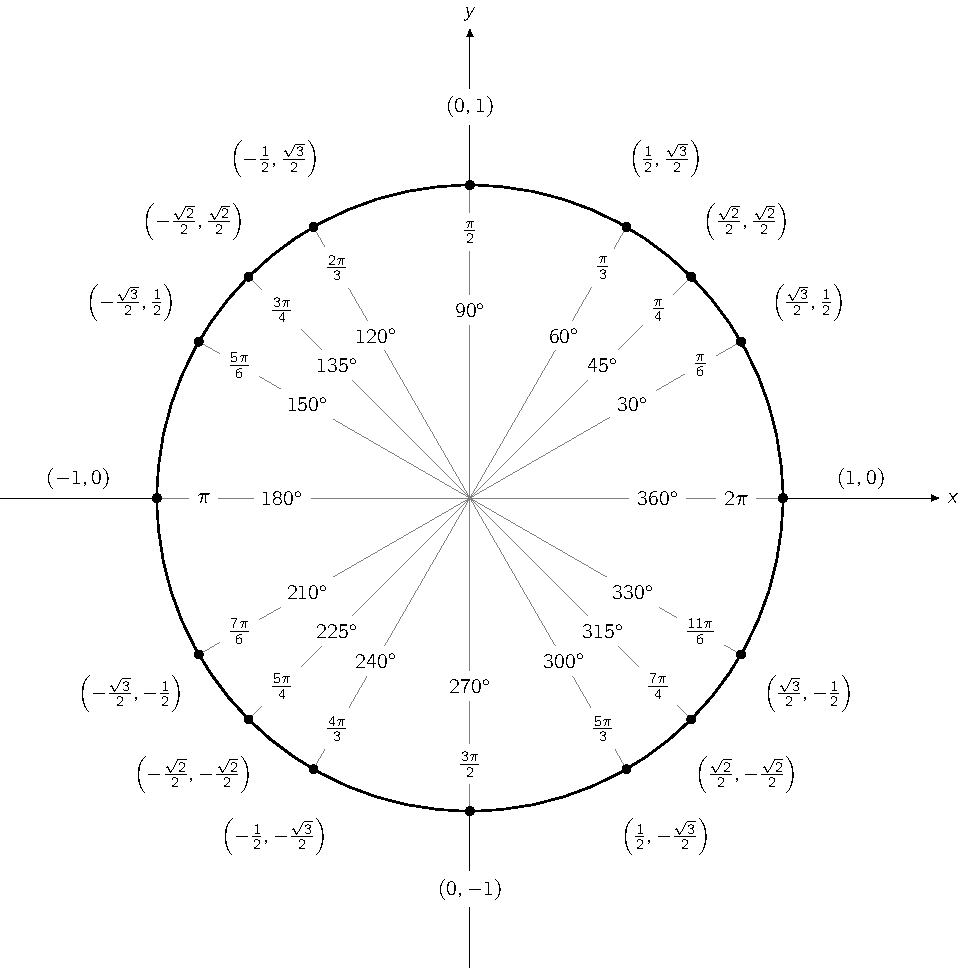
\includegraphics[scale=1]{MATH_1060_Section_1-4_Unit_Circle.pdf}
\end{center}

\newpage

\textbf{The Pythagorean Theorem.} The Pythagorean theorem is useful to remember when working with trig functions.

\vspace{3mm}

\boxenv{Pythagorean Theorem.}{For a right triangle with legs $a$ and $b$ and hypotenuse $c$, we always have that $$a^2+b^2=c^2.$$
\vspace{-6mm}}

\vspace{3mm}

\Example Find $\cos\theta$ and $\tan\theta$ given that $\sin\theta=\disp\frac{3}{5}$ and $\theta\in\ls\frac{\pi}{2},\pi\rs$.

\vspace{40mm}

\textbf{Trigonometric Identities.} Several trigonometric identities can often be useful to manipulate trigonometric functions.
\begin{itemize}
	\item \textbf{Pythagorean Identities.}
	\begin{align*}
	\sin^2\theta + \cos^2\theta &= 1 \\
	1+\tan^2\theta &= \sec^2\theta \\
	1+\cot^2\theta &= \csc^2\theta \\
	\end{align*}
	\item \textbf{Double-Angle Identities.}
	\begin{align*}
	\sin 2\theta &= 2\sin\theta\cos\theta \\
	\cos 2\theta &= \cos^2\theta-\sin^2\theta \\
	\end{align*}
	\item \textbf{Half-Angle Identities.}
	\begin{align*}
	\cos^2\theta &= \frac{1+\cos 2\theta}{2} \\
	\sin^2\theta &= \frac{1-\cos 2\theta}{2} \\
	\end{align*}
\end{itemize}

\newpage 

\textbf{Facts about the Trig Functions.}

\vspace{5mm}

\boxenv{Definition.}{A function is called \textbf{periodic} if there exists $p\in\R$, $p\neq 0$, such that $f(x+p)=f(x)$ for all $x$ in the domain of $f$.}

\vspace{5mm}

By definition, a periodic function is never one-to-one.

\begin{center}
\begin{minipage}{.48\textwidth}
\begin{center}
		\fbox{$y=\sin x$}
		
		\vspace{3mm}
            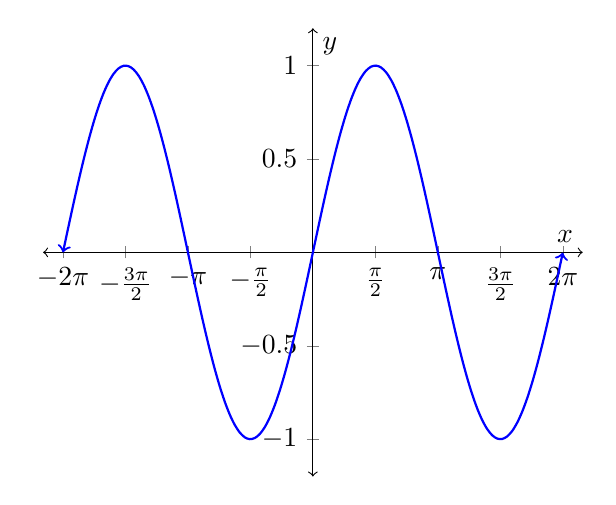
\begin{tikzpicture}
                \begin{axis}[
                	axis x line=middle,
                	xmax=2*pi+.5, xmin=-2*pi-.5,
                	axis y line=center,
                	ymax=1.2, ymin=-1.2,
                	axis line style={<->},
                	xlabel=$x$,ylabel=$y$,
                	xtick={-2*pi,-3*pi/2,-pi,-pi/2,0,pi/2,pi,3*pi/2,2*pi},
                	xticklabels={$-2\pi$,$-\frac{3\pi}{2}$,$-\pi$,$-\frac{\pi}{2}$,0,$\frac{\pi}{2}$,$\pi$,$\frac{3\pi}{2}$,$2\pi$}
                    ]
                    \addplot[name path=f,smooth,domain=-2*pi:2*pi,color=blue,samples=100,<->,thick] {sin(deg(x))};
%                    \addplot[name path=f,smooth,domain=-0.5*pi:0.5*pi,color=red,samples=100,ultra thick] {sin(deg(x))};   
                \end{axis}
            \end{tikzpicture}
            
            \textbf{domain:} $\R$\\
            \textbf{range:} $\left[-1,-1\right]$\\
            \textbf{period:} $2\pi$
        \end{center}
\end{minipage}%
\begin{minipage}{.04\textwidth}
 \phantom{wheeeee!}
\end{minipage}%
\begin{minipage}{.48\textwidth}
\begin{center}
		\fbox{$y=\cos x$}
		
		\vspace{3mm}
            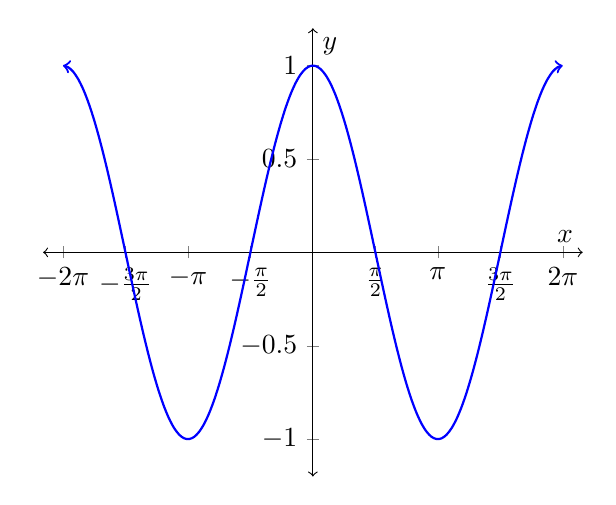
\begin{tikzpicture}
                \begin{axis}[
                	axis x line=middle,
                	xmax=2*pi+.5, xmin=-2*pi-.5,
                	axis y line=center,
                	ymax=1.2, ymin=-1.2,
                	axis line style={<->},
                	xlabel=$x$,ylabel=$y$,
                	xtick={-2*pi,-3*pi/2,-pi,-pi/2,0,pi/2,pi,3*pi/2,2*pi},
                	xticklabels={$-2\pi$,$-\frac{3\pi}{2}$,$-\pi$,$-\frac{\pi}{2}$,0,$\frac{\pi}{2}$,$\pi$,$\frac{3\pi}{2}$,$2\pi$}
                    ]
                    \addplot[name path=f,smooth,domain=-2*pi:2*pi,color=blue,samples=100,<->,thick] {cos(deg(x))};
%                    \addplot[name path=f,smooth,domain=-0.5*pi:0.5*pi,color=red,samples=100,ultra thick] {sin(deg(x))};   
                \end{axis}
            \end{tikzpicture}
            
            \textbf{domain:} $\R$\\
            \textbf{range:} $\left[-1,-1\right]$\\
            \textbf{period:} $2\pi$
        \end{center}
\end{minipage}
\end{center}

\vspace{5mm}

\begin{minipage}{.5\textwidth}
\begin{center}
\fbox{$y=\tan x$}

\vspace{3mm}

            \textbf{domain:} $\R \setminus \left\{\frac{\pi}{2}+n\pi\right\}$\\
            \textbf{range:} $\R$\\
            \textbf{period:} $\pi$
            
            \end{center}
            \vspace{3mm}
            
            Note the vertical asymptotes where $\cos x=0$, i.e.\ at $x=\frac{\pi}{2},\frac{3\pi}{2},\dots$
\end{minipage}%
\begin{minipage}{.5\textwidth}
\begin{center}
            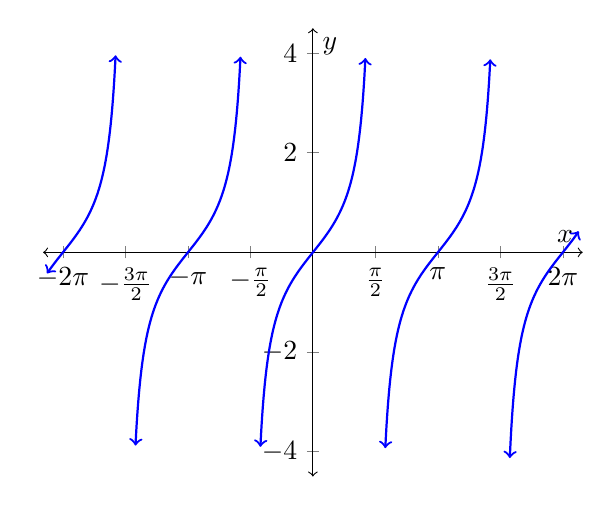
\begin{tikzpicture}
                \begin{axis}[
                	axis x line=middle,
                	xmax=2*pi+.5, xmin=-2*pi-.5,
                	axis y line=center,
                	ymax=4.5, ymin=-4.5,
                	axis line style={<->},
                	xlabel=$x$,ylabel=$y$,
                	xtick={-2*pi,-3*pi/2,-pi,-pi/2,0,pi/2,pi,3*pi/2,2*pi},
                	xticklabels={$-2\pi$,$-\frac{3\pi}{2}$,$-\pi$,$-\frac{\pi}{2}$,0,$\frac{\pi}{2}$,$\pi$,$\frac{3\pi}{2}$,$2\pi$}
                    ]
                    \addplot[name path=f,smooth,domain=-2*pi-.4:-4.96,color=blue,samples=100,<->,thick] {tan(deg(x))}; 
                	\addplot[name path=f,smooth,domain=-4.46:-1.82,color=blue,samples=100,<->,thick] {tan(deg(x))};      
                	\addplot[name path=f,smooth,domain=-1.32:1.32,color=blue,samples=100,<->,thick] {tan(deg(x))};      
                	\addplot[name path=f,smooth,domain=1.82:4.46,color=blue,samples=100,<->,thick] {tan(deg(x))};      
                	\addplot[name path=f,smooth,domain=4.95:2*pi+.4,color=blue,samples=100,<->,thick] {tan(deg(x))};      
%                    \addplot[name path=f,smooth,domain=-2*pi:2*pi,color=blue,samples=100,<->,thick] {tan(deg(x))};               
                     \end{axis}
            \end{tikzpicture}
        \end{center}
\end{minipage}

\newpage

\begin{center}
\renewcommand{\arraystretch}{1.5}
\begin{tabular}{|c|c|c|c|}
\hline
\rowcolor[HTML]{EFEFEF} 
       \textbf{function} & \textbf{domain} & \textbf{range} & \textbf{period} \\ \hline
$\sin\theta$    &  $\R$      & $[-1,1]$      &  $2\pi$      \\ \hline
$\cos\theta$  &  $\R$     & $[-1,1]$      & $2\pi$       \\ \hline
$\tan\theta$ &  $\R\setminus\{\frac{\pi}{2}+n\pi\} $    &  $\R$     &  $\pi$     \\ \hline  
\end{tabular}

\vspace{5mm}
\begin{tabular}{|c|c|c|c|}
\hline
\rowcolor[HTML]{EFEFEF} 
       \textbf{function} & \textbf{domain} & \textbf{range} & \textbf{period} \\ \hline      
$\csc\theta$    &  $\R\setminus\{\pi+n\pi\}$      & $(-\infty,-1]\cup[1,\infty]$      &  $2\pi$      \\ \hline
$\sec\theta$  &  $\R\setminus\{\frac{\pi}{2}+n\pi\}$     & $(-\infty,-1]\cup[1,\infty]$     & $2\pi$       \\ \hline
$\cot\theta$ &  $\R\setminus\{\pi+n\pi\} $    &  $\R$     &  $\pi$     \\ \hline
\end{tabular}
\end{center}

\vspace{3mm}

\Example Solve the following equation defined on the interval $\ls 0,2\pi\rs$.
$$\sin^2\theta+2\sin\theta+2=1$$

\vspace{30mm}

\Example Solve the following equation defined on the interval $\ls 0,2\pi\rs$.
$$\tan^2x-\tan x=0$$

\vspace{30mm}

\subsection*{Inverse Trigonometric Functions}

The trig functions act on \textit{angles} and return \textit{ratios}. If we wanted a function that instead acts on a \textit{ratio} and returns an \textit{angle}, we would need an \textbf{inverse trig function}. Note that trig functions are periodic, so they are not one-to-one and thus do not have inverses. However, we can define an inverse trig function if we \textit{restrict the domain} of a trig function.

\newpage

Consider the sine function $y=\sin x$. We can see that it is not one-to-one on its domain $\R$. 

\begin{center}
            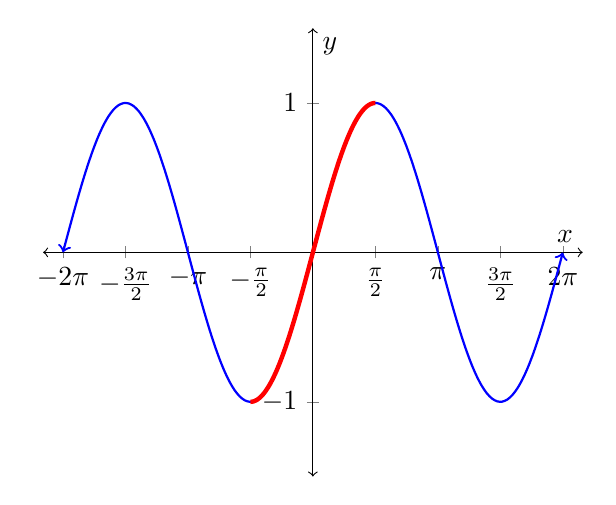
\begin{tikzpicture}
                \begin{axis}[
                	axis x line=middle,
                	xmax=2*pi+.5, xmin=-2*pi-.5,
                	axis y line=center,
                	ymax=1.5, ymin=-1.5,
                	axis line style={<->},
                	xlabel=$x$,ylabel=$y$,
                	xtick={-2*pi,-3*pi/2,-pi,-pi/2,0,pi/2,pi,3*pi/2,2*pi},
                	xticklabels={$-2\pi$,$-\frac{3\pi}{2}$,$-\pi$,$-\frac{\pi}{2}$,0,$\frac{\pi}{2}$,$\pi$,$\frac{3\pi}{2}$,$2\pi$}
                    ]
                    \addplot[name path=f,smooth,domain=-2*pi:2*pi,color=blue,samples=100,<->,thick] {sin(deg(x))};
                    \addplot[name path=f,smooth,domain=-0.5*pi:0.5*pi,color=red,samples=100,ultra thick] {sin(deg(x))};   
                \end{axis}
            \end{tikzpicture}
        \end{center}
        
However, it is one-to-one on the interval $\ls-\frac{\pi}{2},\frac{\pi}{2}\rs$ (highlighted in red) and spans the values of $\ls-1,1\rs$. We can then define the inverse sine function $f(x)=\arcsin x$ with domain $\ls-1,1\rs$ and range $\ls-\frac{\pi}{2},\frac{\pi}{2}\rs$.

\vspace{5mm}

\boxenv{Remark.}{Notationally, inverse trig functions may be expressed as
$$\sin^{-1}x=\arcsin x.$$
Note that the $-1$ in the inverse trig function notation is \textbf{not} a negative exponent.
$$\sin^{-1}x\neq\frac{1}{\sin x}=\csc x$$
\vspace{-5mm}}

\vspace{5mm}

\boxenv{Remark.}{The following are equivalent expressions.
$$y=\arcsin x \Longleftrightarrow \sin y=x$$
\vspace{-6mm}}

\vspace{7mm}

\begin{minipage}{.33\textwidth}
\begin{center}
\fbox{Inverse Sine}

\vspace{3mm}

            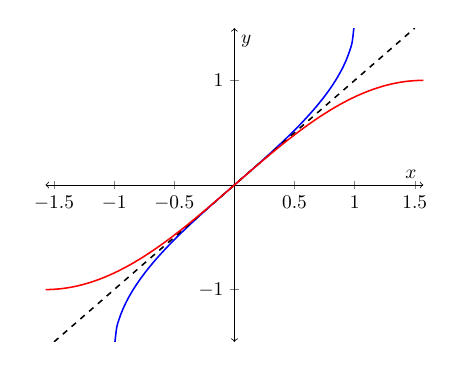
\begin{tikzpicture}[scale=.7]
                \begin{axis}[
                	axis x line=middle,
                	xmax=0.5*pi, xmin=-0.5*pi,
                	axis y line=center,
                	ymax=1.5, ymin=-1.5,
                	axis line style={<->},
                	xlabel=$x$,ylabel=$y$
                    ]
                    \addplot[name path=f,smooth,domain=-1:1,color=blue,samples=100,thick] {asin(x)/180*pi};
                    \addplot[name path=f,smooth,domain=-1.5:1.5,color=black,dashed,samples=100,thick] {x};
                    \addplot[name path=f,smooth,domain=-0.5*pi:0.5*pi,color=red,samples=100, thick] {sin(deg(x))};   
                \end{axis}
            \end{tikzpicture}
        \end{center}
\end{minipage}%
\begin{minipage}{.33\textwidth}
\begin{center}
\fbox{Inverse Cosine}

\vspace{3mm}

            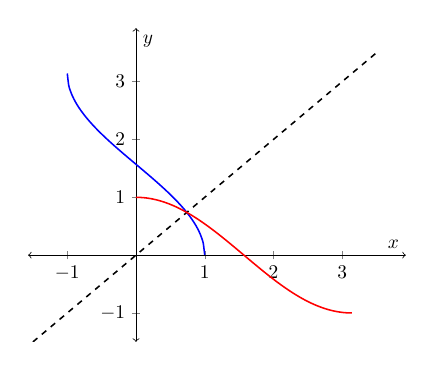
\begin{tikzpicture}[scale=.7]
                \begin{axis}[
                	axis x line=middle,
                	xmax=1.25*pi, xmin=-0.5*pi,
                	axis y line=center,
                	ymax=1.25*pi, ymin=-1.5,
                	axis line style={<->},
                	xlabel=$x$,ylabel=$y$
                    ]
                    \addplot[name path=f,smooth,domain=-1:1,color=blue,samples=100,thick] {acos(x)/180*pi};
                    \addplot[name path=f,smooth,domain=-1.5:3.5,color=black,dashed,samples=100,thick] {x};
                    \addplot[name path=f,smooth,domain=0:pi,color=red,samples=100, thick] {cos(deg(x))};   
                \end{axis}
            \end{tikzpicture}
        \end{center}
\end{minipage}%
\begin{minipage}{.33\textwidth}
\begin{center}
\fbox{Inverse Tangent}

\vspace{3mm}

            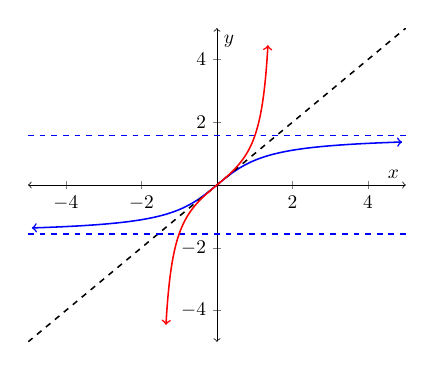
\begin{tikzpicture}[scale=.7]
                \begin{axis}[
                	axis x line=middle,
                	xmax=5, xmin=-5,
                	axis y line=center,
                	ymax=5, ymin=-5,
                	axis line style={<->},
                	xlabel=$x$,ylabel=$y$
                    ]
                    \addplot[name path=f,smooth,domain=-4.9:4.9,color=blue,samples=100,<->,thick] {atan(x)/180*pi};
                    \addplot[name path=f,smooth,domain=-5:5,color=black,dashed,samples=100,thick] {x};
                    \addplot[name path=f,smooth,domain=-5:5,color=blue,dashed,samples=100,thick] {pi/2};
                    \addplot[name path=f,smooth,domain=-5:5,color=blue,dashed,samples=100,thick] {-pi/2};
                    \addplot[name path=f,smooth,domain=-1.35:1.35,color=red,samples=100,<->, thick] {tan(deg(x))};   
                \end{axis}
            \end{tikzpicture}
        \end{center}
\end{minipage}

\newpage

Inverse trig functions are achieved by forcing the original functions to be one-to-one through \textbf{domain restrictions}. The restricted domain of the original trig function becomes the range of the inverse trig function.

\begin{center}
\renewcommand{\arraystretch}{1.5}
\begin{tabular}{|c|c|c|}
\hline
\rowcolor[HTML]{EFEFEF} 
   \textbf{function}    & \textbf{domain} & \textbf{range} \\ \hline
$\arcsin\theta$ & $[-1,1]$      & $[-\frac{\pi}{2},\frac{\pi}{2}]$  \\ \hline
$\arccos\theta$ & $[-1,1]$      & $[0,\pi]$    \\ \hline
$\arctan\theta$ & $\R$       & $(-\frac{\pi}{2},\frac{\pi}{2})$        \\ \hline
\end{tabular}
\end{center}

\begin{center}
\renewcommand{\arraystretch}{1.5}
\begin{tabular}{|c|c|c|}
\hline
\rowcolor[HTML]{EFEFEF} 
\textbf{function} & \textbf{domain} & \textbf{range} \\ \hline
 arccsc $\theta$ & $(-\infty,-1]\cup[1,\infty)$       & $[-\frac{\pi}{2},0)\cup(0,\frac{\pi}{2}]$     \\ \hline
 arcsec $\theta$ & $(-\infty,-1]\cup[1,\infty)$        & $[0,\frac{\pi}{2})\cup(\frac{\pi}{2},\frac{3\pi}{2}]$       \\ \hline
arccot $\theta$ &  $\R$      & $(0,\pi)$      \\ \hline
\end{tabular}
\end{center}

\Example Evaluate the following expressions.

\begin{enumerate}
	\item[\tc{1}] $\arccos\lp\disp\frac{1}{2}\rp$
	
	\vspace{15mm}
	
	\item[\tc{2}] $\arccos\lp-\disp\frac{1}{\sqrt{2}}\rp$
	
	\vspace{15mm}
	
	\item[\tc{3}] $\cos\lp\arccos(-1)\rp$
	
	\vspace{15mm}
	
	\item[\tc{4}] $\arccos\lp\cos\lp\disp\frac{7\pi}{6}\rp\rp$
\end{enumerate}

\newpage

\Example Use a right triangle to simplify the expression. Assume $x>0$.
$$\sin\lp\arccos\lp\disp\frac{x}{2}\rp\rp$$
\end{document}